
\chapter{General Description}


\section{System Overview}

\gls{utc}

The processes of the system are shown in \abb{fig:system}. The ASW shall communicate with the GS, exchanging telecommands and telemetry. The ASW will handle the commands in two different ways. Concerning the movements of the rover itself, the commands will be executed by the ASW, while all commands for the grip arm and the camera are relayed to a different controller system, which is already implemented. Additionally, the voltage of the battery and the current of the motor are measured via an ADC.\\

\begin{figure}[H]
\centering
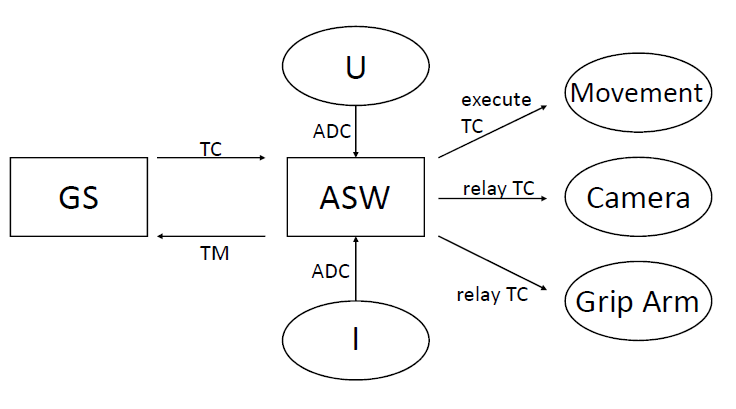
\includegraphics[scale=0.7]{system.PNG}
\caption{Functionality of the system.}
\label{fig:system}
\end{figure}


The requirements for the ASW are grouped according to its main functions. Four parts have been identified:
\begin{itemize}
\item Modes
\item Initialization
\item Commands
\item Telemetry
\end{itemize}

Modes is responsible for controlling the transitions between the different modes that the ASW has. The initialization sets up the system after its start. Commands includes receiving and executing/relaying of the received commands from the ground station. Telemetry is responsible for monitoring the system and sending a telemetry message.


\section{Function and Purpose}
The ASW shall be able to receive commands from the ground station. Those commands have to be split in the parts concerning the movement, the grip arm and the camera. Commands for the movement shall be executed, while commands for the other two devices are passed on to separate controllers. Additionally, the ASW shall monitor the voltage of the battery and the current taken by the motor. The battery voltage shall be included in a telemetry set, sent back to the ground station.\\


\section{Constraints}

The development of the ASW is mainly constrained by the fact, that the entire hardware interacting with the SW is already chosen and present. Additionally, the other software parts controlling the rover movements, the grip arm and the camera are already implemented as well as the ground station. For that reason, the developed ASW has to be highly orientated towards those existing parts as no changes are possible in the surrounding systems anymore.